\subsection{Root and Copy Protection} \label{subsection:android-copyroot}
\begin{itemize}
  \item root is getting total control over system
  \item comes from linux
  \item used to circumvent limitations by carrier, manufacturers, extend system
  \item not approved but vulnerabilities used to exploit, often and many exploited
  \item easy even for non techies, videos tutorials tools
  \item su user helps to handle
  \item risks, bricking
  \item root voids copy protection since access to asec folder can be gained, effective when root was hard to get
\end{itemize}
\begin{figure}[h]
    \centering
    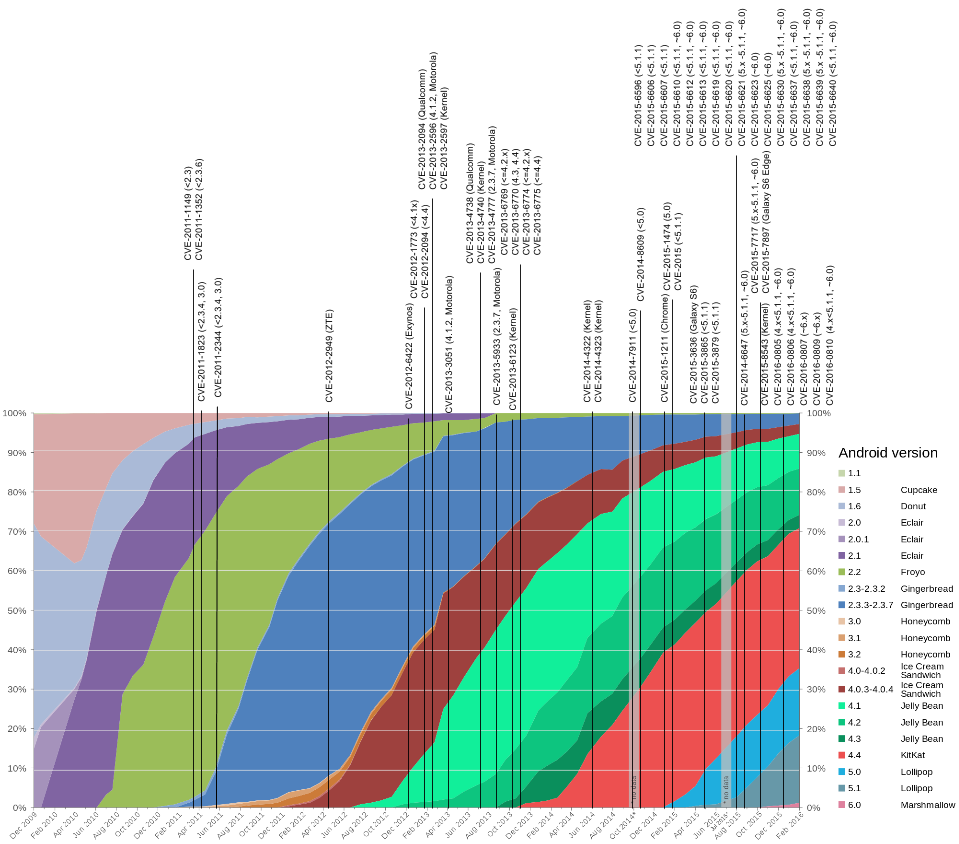
\includegraphics[width=1\textwidth]{data/timeline.png}
    \caption{Timeline of market share of evolving Android versions and dates of root exploits recorded \cite{distributionRoot} \cite{androidVulnerabilities} \cite{cveAndroidPriv} \cite{cveDetails}}
    \label{fig:root}
\end{figure}
